\documentclass[letterpaper, notitlepage, 11pt]{article}
\usepackage{fullpage}
\usepackage{graphicx}
\usepackage{hyperref}
\usepackage{url}
\usepackage{titling}

% This is here so we can have a fancier title page than LaTeX gives us by default
\newcommand{\department}[1]{%
  \gdef\dept{#1}}
\newcommand{\dept}{}
\renewcommand{\maketitlehookd}{%
\par\noindent \dept }

\title{
	smrt: A 3D Media Center User Interface
	\\
	Design Decisions
}
\author{
	Cory Maccarrone  \\ {\small \href{mailto:Cory.Maccarrone@colorado.edu}{Cory.Maccarrone@colorado.edu}}
	\and
	Daniel Seikaly   \\ {\small \href{mailto:Daniel.Seikaly@colorado.edu}{Daniel.Seikaly@colorado.edu}}
	\and
	Evan Sheehan     \\ {\small \href{mailto:Wallace.Sheehan@gmail.com}{Wallace.Sheehan@gmail.com}}
	\and
	David Trowbridge \\ {\small \href{mailto:trowbrds@gmail.com}{trowbrds@gmail.com}}
}
\date{December 2, 2005}
\department{
\begin{center}
	CSCI 4308-4318. Software Engineering Project 1 \& 2 \\
	Department of Computer Science \\
	University of Colorado at Boulder \\
	2005-2006 \\
	\vspace{1.5em}
	Sun Microsystems \\
	Santa Clara, CA \\
	\vspace{1em}
	Paul Byrne \\
	{\small \href{mailto:Paul.Byrne@Sun.COM}{Paul.Byrne@Sun.COM}} \\
	\vspace{1em}
	Hideya Kawahara \\
	{\small \href{mailto:Hideya.Kawahara@Sun.COM}{Hideya.Kawahara@Sun.COM}}
\end{center}
}


\begin{document}
\maketitle

\raggedbottom

\pagenumbering{roman}

\hspace{1em}
\pagebreak

\tableofcontents

\pagebreak
\hspace{1em}
\pagebreak

\pagenumbering{arabic}

\documentclass[letterpaper, notitlepage, 11pt]{article}
\usepackage[body={6in, 8in}, left=1in, right=1in, top=1in, bottom=1in]{geometry}
\usepackage{fancyhdr}

\pagestyle{empty}

\begin{document}
\documentclass[letterpaper, notitlepage, 11pt]{article}
\usepackage[body={6in, 8in}, left=1in, right=1in, top=1in, bottom=1in]{geometry}
\usepackage{fancyhdr}

\pagestyle{empty}

\begin{document}
\documentclass[letterpaper, notitlepage, 11pt]{article}
\usepackage[body={6in, 8in}, left=1in, right=1in, top=1in, bottom=1in]{geometry}
\usepackage{fancyhdr}

\pagestyle{empty}

\begin{document}
\input{../lib/project-proposal}
\end{document}

\end{document}

\end{document}

\section{Introduction}
As a company, one of Sun Microsystems' objectives is to innovate the world of
computing. To this end, Sun created Project Looking Glass to explore the field
of 3D user interfaces and determine what improvements in user interaction can be
made by taking advantage of the third dimension. Through Project Looking Glass,
Sun hopes to begin redefining how people think of user interfaces and create
useful design concepts for a 3D computing environment. At the moment, Looking
Glass consists of a framework for developing 3D applications and a desktop
environment to run them alongside existing 2D applications.

The goal of this project, code named \textit{smrt}, is to create a user
interface for a home media center along the lines of TiVo, but using 3D user
interface elements within the Looking Glass environment. The name \textit{smrt}
-- pronounced ``smeert'' -- is the Czech word for ``death,'' and was primarily
chosen because it is fun to say and spell.

Figure \ref{figure:concept} presents a conceptual diagram of the overall
system.  This diagram shows how \textit{smrt} interacts with its software and
hardware environment. At the most basic level, \textit{smrt} allows a user to
browse through and play media, as well as watch or record a TV show.  To control
the system, a simple input device such as keyboard or remote control is used.
Note that this project is focused on the user interface; actual functionality
may not exist.

\begin{figure}[htb]
\centering
\includegraphics[width=4in]{figures/conceptual_overview}
\caption{Conceptual overview of the \textit{smrt} project\label{figure:concept}}
\end{figure}


As a result of this project's goal, \textit{smrt} employs some unusual user
interfaces.  This document purposes to expose the innermost workings of the
developers's minds and clarify the decisions made regarding \textit{smrt}'s
unusual user interface.  Primarily, we are concerned with the system of menus
used by \textit{smrt} to provide the media center functionality to the user.
We will also spend some time discussing menu configuration, as this is
also an aspect of how users may interact with \textit{smrt}.

\section{Menus}
\textit{smrt}'s interface is composed mostly of menus -- specifically: the
ring menu, the arc menu, and the cityscape menu.  Each menu is intended for use
in specific types of situations, but share certain themes with each other.  The
common properties of these menus help to tie the interface together and
increase the user's comfort.

The user's location in the menu is indicated by the size of the menu items,
\textit{i.e.} the largest menu item is the currently selected one.  The
remaining items are displayed exponentially smaller as a function of their
distance from the selected one.  This sizing scheme results in easy
identification of the user's current position in any menu.

\subsection{The Ring Menu}
The ring menu (Figure \ref{fig:ringmenu}) is designed for small numbers of
items.  It displays all of the menu items in a circle.  This layout allows the
user to see all available menu items at once, making it easier to find the
desired item.  This property is only true for menus with relatively few items.
With too many items in the menu, the items begin to obscure each other, making
it more difficult to find what one is looking for.

\begin{figure}[htb]
\centering
\includegraphics[width=4in]{figures/circle_menu_1}
\caption{A ring menu\label{fig:ringmenu}}
\end{figure}

The ring menu's circular nature also makes accessing items quicker.  From any
given item in the menu there are at most $n \over 2$ button presses to select
any other item, where $n$ is the number of items in the menu.

\subsection{The Arc Menu}
The arc menu is used for displaying additional information besides the contents
of a menu.  Figure \ref{fig:arcmenu} shows an arc menu displaying the current
show on a television channel with the program title and additional schedule
information beneath it.  Due to the amount of space available to the left of the
menu items, the arc menu is useful when information beyond an icon and name is
desired for a menu item.  A television program guide -- as in Figure
\ref{fig:arcmenu} -- is an excellent example of such a case.  Each item
represents a TV channel; to the left of each item is displayed what is currently
showing on the channel as well as the immediate program schedule for the
channel.

\begin{figure}[htb]
\centering
\includegraphics[width=4in]{figures/arc_menu}
\caption{An arc menu\label{fig:arcmenu}}
\end{figure}

\subsection{The Cityscape Menu}
Inspired by the file browser from the movie \textit{Jurassic Park}, the
cityscape menu (Figure \ref{fig:cityscape}) is designed to manage very large
numbers of menu items.  Because \textit{smrt} has to manage personal media
collections it must elegantly navigate large collections of media; people may
have thousands of songs or videos stored on their hard drives, and they do not
want to have to traverse their entire collection alphabetically just to listen
to Yes.  The cityscape menu provides non-linear access to the items in the menu;
thus, it reduces the number of button presses to access items.

\begin{figure}[htb]
\centering
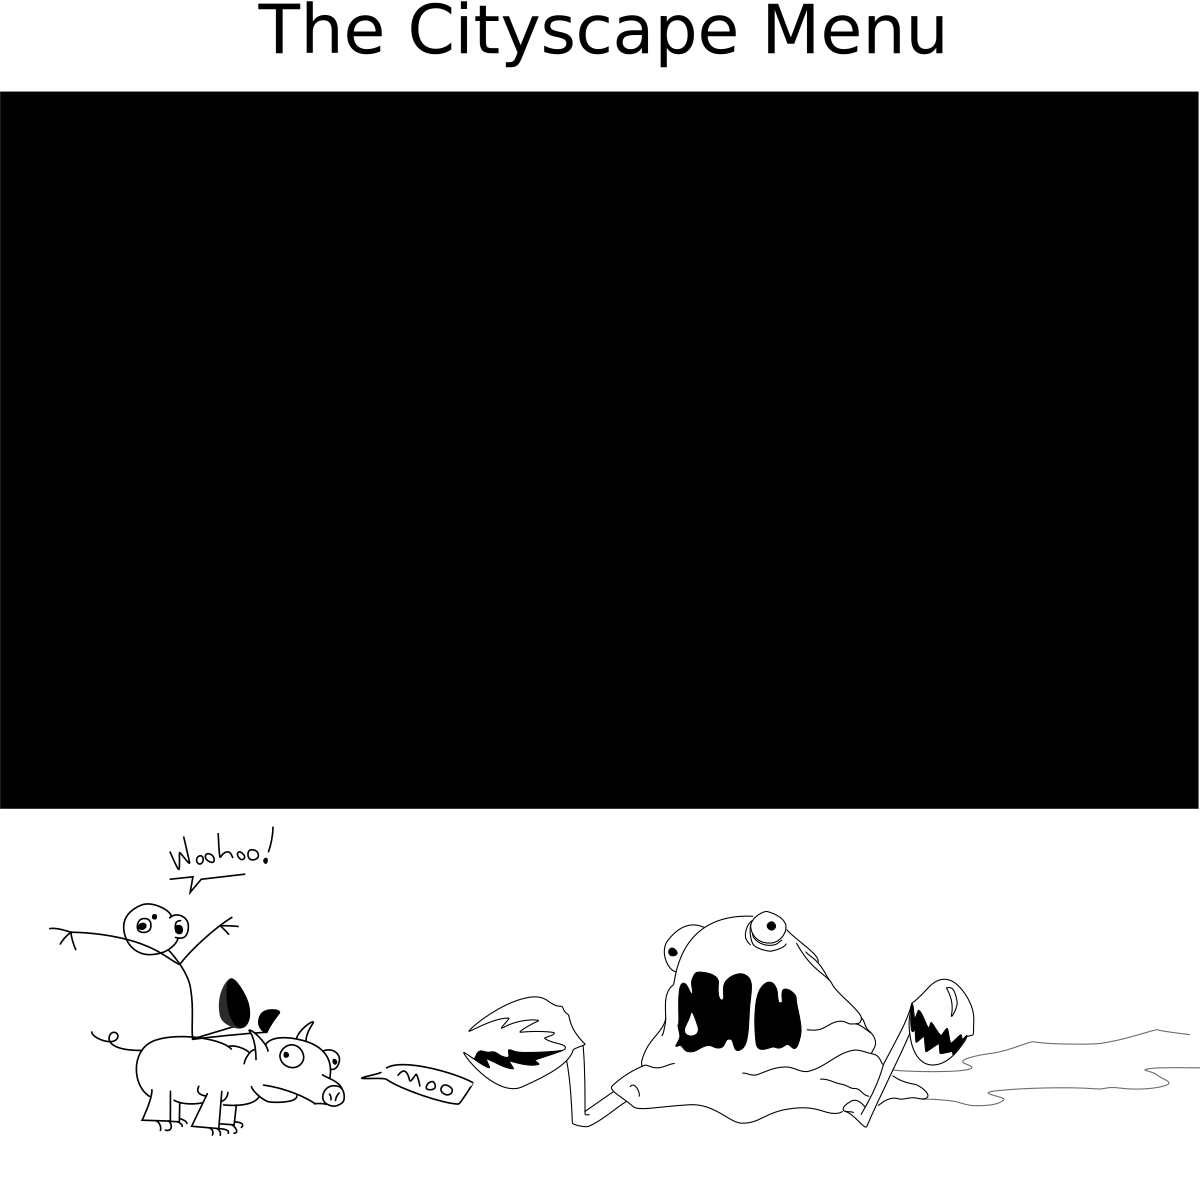
\includegraphics[width=4in]{figures/cityscape}
\caption{A cityscape menu\label{fig:cityscape}}
\end{figure}

The cityscape menu also implies some kind of logical relationship between one
menu and the next.  Each item is allowed to contain sub-items that are displayed
on top of their container.  If an item containing sub-items is activated, the
menu zooms in on the item and its sub-items are displayed as another cityscape
menu.  An item in either a ring or arc menu may bring up an application just as
easily as it might bring up another menu; nothing about the items in these menus
suggests one type of behavior over the other.  But in the cityscape menu, if an
item has other, smaller items sitting on top, you know it will bring up another
menu.  This property makes the cityscape menu ideal for browsing files -- when
activating a directory, one expects another menu; when activating a file, one
expects an application that displays the file.  When used as a file browser,
items representing directories will display their contents on top of themselves,
files will have nothing on top, and based on these visual cues the user will
always know what to expect.

\section{Files}
A more esoteric aspect of \textit{smrt}'s interface is its configuration files.
These files, written in XML, control \textit{smrt}'s behavior: they define menu
hierarchies, actions taken by menu items, and applications used for media
playback.  Thus, if a user is not satisfied with the default configuration, he
or she may change \textit{smrt}'s behavior by editing these files.  No two home
theaters are identical; for this reason \textit{smrt}'s interface is completely
configurable.

This project's purpose, however, is not to be configured; it's purpose is to
provide media center functionality.  So this facet of the interface is one which
will be used minimally.  Some amount of configuration will be necessary for most
systems -- most users will at least need to configure \textit{smrt} to find the
music or videos stored on their computer.  For these users, modifying the
default configuration files will suffice.  Others may choose to redefine the menu
system in the interface using these XML files.

\section{Summary}
\textit{smrt}'s primary interface uses a system of menus.  Each menu was
designed for specific use cases based on the number of items contained in
each menu.  Each menu takes advantage of its 3D environment to improve usability
over 2D menus.  In addition to its menus, \textit{smrt} allows the user to
interact with it at a lower level using its configuration files.  Because the
configuration files do not pertain to \textit{smrt}'s primary task, and not
every user enjoys configuring software, the required amount of interaction with
this interface is kept to a minimum.

\end{document}
